\chapter{Architecture d'Entreprise}
\label{ch:EA}

\section{Notions fondamentales de l'Architecture d'Entreprise}

Comme précédemment exposé dans notre problématique de recherche (cf. chapitre 
\ref{ch:problematique}), nos travaux se sont d'abord portés sur la modélisation 
et la simulation du SI des Smart Grids. Cependant, le SI est sensé répondre de 
manière pertinente aux besoins de l'entreprise et implémenter efficacement sa 
stratégie. Avant toute simulation, nous devons donc de facto prendre en compte 
la stratégie de l'entreprise et ses objectifs métier et la mettre en cohérence 
avec le SI qui l'implémente.

L'alignement métier/SI est au cœur de l'EA, une discipline à part entière qui 
traite le SI en le corrélant au reste de l'entreprise. En effet, l'EA offre une 
vision globale des composants de l'entreprise tels que les processus métier, les 
parties prenantes, les informations, les fonctions, les applications 
informatiques, les infrastructures techniques. 

Nous consacrons cette première partie de l'état de l'art à l'EA en commençant 
par définir les termes de SI et d'EA. 
 
\subsection{Terminologie}
	
\subsubsection{Système d'Information}

Selon Robert Reix, le SI est «~un ensemble organisé de ressources : matériel, 
logiciel, personnel, données, procédures permettant d'acquérir, de traiter, de 
stocker des informations (sous forme de donnée, textes, images, sons, etc.) dans 
et entre des organisations~» \cite{reix1995systemes}.

Nous adoptons cette définition car elle a l'avantage de ne pas réduire le SI 
d'une organisation à son système informatique. Le système informatique est 
constitué de l'ensemble du patrimoine matériel (hardware) et applicatif 
(software) de la dite 
organisation et a pour objectif d'automatiser le traitement de l'information. 
Nous adoptons l'acronyme IT (\textit{Information Technologies}) pour le 
différencier du SI.

On suppose souvent que les SI sont totalement informatisés et c'est une des 
raisons qui mènent à confondre SI et \ Cependant, le SI comprend non seulement 
le système informatique mais aussi des ressources humaines telles que les 
partenaires ou le personnel et des ressources matérielles comme les procédures 
de gestion ou encore le savoir-faire métier.

\subsubsection{Architecture d'Entreprise}

Selon Zachman, une architecture d'entreprise est «~un ensemble pertinent 
d'artefacts de conception ou de représentations descriptives pour décrire une 
entreprise de manière à ce cette entreprise soit créée en respectant certaines 
exigences et à ce qu'elle soit facilement maintenue tout au long de son cycle de 
vie~» \cite{zachman1997enterprise}. 

Zachman voit ainsi dans l'architecture un gage de qualité et de maintenabilité. 
L'EA revient à appliquer à l'entreprise les principes de l'architecture telle 
qu'elle est pratiquée dans de nombreuses autres disciplines comme par exemple 
l'architecture du bâtiment. Construire une maison en procédant chambre par 
chambre sans plan d'architecture général peut en effet mener à un résultat peu 
probant. De même, le développement préalable d'une organisation sans 
architecture de référence risque de mener à une duplication de ses ressources et 
altère par conséquent son efficacité, sa cohérence interne rend fastidieuse 
toute entreprise de changement \cite{zachman1997enterprise} 
\cite{bernard2012introduction}. 

Il est important de noter que le terme architecture d'entreprise peut prêter à 
confusion car il est à la fois utilisé pour désigner (1) l'activité de 
conception d'une architecture i.e. la description des éléments composant 
l'organisation en question et leurs relations mais aussi (2) l'ensemble des 
artefacts résultant de cette activité. Pour éviter toute confusion, nous 
désignons l'activité de conception par l'acronyme EA et le résultat de cette 
activité, c'est-à-dire les artefacts qui en sont issus, comme étant 
l'architecture de l'entreprise. L'EA est apparue en tant que discipline dans 
les années 1980 suite à l'informatisation accrue des entreprises mais son 
périmètre ne cesse d'évoluer depuis. La section suivante écrit les raisons et 
les grandes étapes de cette évolution. 

%%S'agissant du terme «~entrerprise~», Scott Bernard 
%\cite{bernard2012introduction} y réfère comme une organisation ou une 
%sous-partie d'une organisation qui poursuit des objectifs 
%%communs, en s'appuyant sur les mêmes processus et en utilisant les mêmes 
%%ressources. Une entreprise peut être publique ou privée, avoir ou pas un but 
%lucratif. 

\subsection{Évolution de l'Architecture d'Entreprise}

L'EA est ancrée dans l'architecture de systèmes informatiques
\cite{kappelman2008enterprise}. Mais le périmètre de l'EA ne cesse de s'étendre
en comprenant d'abord l'IT et certains aspects métier de l'entreprise
\cite{winter2006essential}, évoluant ensuite en adressant l'ensemble de
l'entreprise en intégrant sa stratégie et ses processus décisionnels
\cite{ross2006enterprise}, et allant même jusqu'à aborder l'environnement dans
lequel elle évolue \cite{lapalme2012three}.

L'origine de l'EA\footnote{D'après Scott Bernard
\cite{bernard2012introduction}, le terme Architecture d'Entreprise a fait sa
première apparition dans le livre de Steven Spewak intitulé «~Enterprise
Archietcture Planning~:~developing a blueprint for data, applications and
technology~» \cite{spewak1993enterprise}.} remonte en effet aux travaux de
Zachman, souvent considérés comme précurseurs.  Il y propose un cadre
d'architecture pour l'IT \cite{zachman1987framework} afin d'optimiser la
gestion du patrimoine applicatif et de l'infrastructure technique de
l'entreprise. À ses débuts, l'EA se focalise donc sur des artefacts purement IT
(data, logiciels, équipements) pour rationaliser l'utilisation des ressources
informatiques \cite{winter2006essential}, tout en répondant aux besoins métier
de l'entreprise. L'EA est alors guidée par les pratiques de l'ingénierie
logicielle. 

Cependant, l'accroissement de la complexité de l'IT et son rôle de plus en plus
prégnant dans le cœur de métier des entreprises
\cite{ranganathan2005enterprise} ont fait de l'architecture IT une
problématique inhérente à l'ensemble des composants de l'entreprise. Pour y
faire face, l'EA a commencé à inclure quelques aspects métier tels les
processus les acteurs impliqués \cite{winter2006essential}. En intégrant ainsi
des problématiques métier, l'EA ne relève plus de l'architecture IT mais de
l'architecture du SI dans son ensemble.

Pour Scott Bernard, l'EA doit même aller plus loin en intégrant la stratégie de
l'entreprise dans son périmètre pour offrir une vision globale de l'ensemble
des ressources de l'entreprise \cite{bernard2012introduction}. Le terme
«~entreprise~» implique ainsi une vue à haut niveau de l'ensemble de
l'organisation. Le terme «~architecture~» fait référence à la mise en place
d'un cadre structuré et cohérent pour l'analyse, le planning, et le
l'exploitation de toutes les ressources dont dispose l'entreprise pour
atteindre ses objectifs.  

Enfin, certains auteurs insistent sur le fait que l'entreprise évolue dans un
environnement inconstant \cite{lapalme2012three}. L'EA doit par conséquence
inclure les relations de l'entreprise avec son environnement pour mesurer
l'impact de ce dernier et faciliter les processus d'adaptation et d'innovation.
Les différentes phases d'évolution de l'EA sont à l'origine de l'apparition de
plusieurs écoles que nous détaillons dans la section suivante. 


\subsection{Écoles de pensée de l'Architecture d'Entreprise} 
\label{Lapalme}

Aucune définition de l'EA n'a été universellement adoptée
\cite{mentz2012comparison} \cite{ranganathan2005enterprise}. Il existe en effet
une pléiade de définitions émanant aussi bien du milieu académique que du
milieu industriel donnant ainsi lieu à plusieurs écoles de pensée. Ce manque de
consensus est du à la nature intrinsèque de l'activité d'EA~:~celle-ci est
régie par un ensemble de préceptes et de bonnes pratiques que l'architecte
reste libre d'adapter au contexte de l'entreprise. 

Il est toutefois possible d'identifier un thème commun à toutes les définitions
proposées~:~l'architecture d'entreprise décrit les composants interdépendants
d'une organisation et guide leurs évolutions \cite{lapalme2012three}. En
revanche, le \textit{périmètre} de cette description ainsi que les
\textit{préoccupations} adressées diffèrent d'une définition à l'autre.

S'agissant du \textit{périmètre}, le terme «~entreprise~» peut couvrir
uniquement l'IT ou s'étendre à tous ses composants humains, stratégiques,
économiques et techniques. Les \textit{préoccupations} sous-jacentes à l'EA
peuvent quant à elles couvrir des objectifs allant de l'optimisation des
investissements dans l'infrastructure technique à l'implémentation de la
stratégie de l'entreprise en passant par l'alignement métier/IT. 

Partant de ce constat, James Lapalme identifie trois écoles de pensée en EA 
\cite{lapalme2012three}~:~l'architecture de l'IT d'entreprise 
(\textit{Enterprise IT Architecting}), l'architecture intégrative de 
l'entreprise 
(\textit{Enterprise Integrating}) et l'architecture de l'entreprise dans son 
environnement (\textit{Enterprise Ecological Adaptation}). Chaque école a son 
propre système de croyance (devise, préoccupations et objectifs, principes et 
postulats).


%\textcolor{red}{Le terme "système de croyances" est vraisemblablement emprunté 
%à la sociologie, j'aime bien l'idée d'utiliser d'autres disciplines pas 
%forcément directement mais Lapalme ne fait pas du tout la référence à la 
%sociologie en parlant de belief system. J'ai une amie qui a un master en socio 
%je peux lui demander une petite référence pour définir exactement ce qu'est un 
%système de croyances. En lisant la préface de Zachman dans le livre de Scott 
%Bernard, on y 
%entrevoit clairement une problématique de catégorie de gens qui croient que la 
%clé de l'architecture c'est la technologie sans tenir compte des 
%problématiques métier. à voir donc. Au pire je supprime simplement le terme 
%«~système de croyances~» mais je trouve ça dommage parce que ça explique pas 
%mal 
%de choses.}

Il est important de noter que cette une catégorisation est épurée voire
idéalisée, dans la mesure où le majorité des auteurs gravitent autour d'une
école plutôt que de se conformer complètement à une seule école.
\textit{Enterprise IT Architecting} réduit le périmètre de l'architecture à
l'IT de l'entreprise.  \textit{Enterprise Integration} adopte une approche
intégrative en incluant toute l'entreprise dans son périmètre, de sa stratégie
métier à la gestion de son patrimoine applicatif. \textit{Enterprise Ecological
Adaptation} inclue l'environnement dans lequel évolue l'entreprise pour en
déterminer les impacts potentiels et mettre en place une stratégie d'adaptation
adéquate. Le tableau \ref{tab:ecolePensee} résume ces écoles de pensée en
termes de devises, objectifs et principes. 

\begin{table}[!ht]
	\setlength{\mytablewidth}{1.1\textwidth}
\setlength{\dashlinedash}{0.5pt}
\setlength{\dashlinegap}{1pt}
\setlength{\arrayrulewidth}{0.5pt}
\begin{adjustbox}{width=\mytablewidth,center}
    \setlength{\mycolwidth}{\dimexpr0.28\mytablewidth-2\tabcolsep\relax}
    \setlength{\myfirstcolwidth}{\dimexpr0.16\mytablewidth-2\tabcolsep\relax}
    \scriptsize
    \begin{tabulary}{\mytablewidth}{@{}>{\bfseries}p{\myfirstcolwidth}p{\mycolwidth}p{\mycolwidth}p{\mycolwidth}@{}}
        %  --------------------------------------------------------------------
        \toprule
        & \centering\textbf{Enterprise IT Architecting} \
        & \centering\textbf{Enterprise Integration} \
		& \centering\textbf{Enterprise Ecological\newline Adaptation}\
        \tabularnewline\midrule
        %  --------------------------------------------------------------------
        \multirow{1}{\myfirstcolwidth}{Devise} \
        & L'architecture d'entreprise raccorde l'IT au métier de l'entreprise \
        & L'architecture d'entreprise lie la stratégie et son exécution \
        & L'architecture d'entreprise est un moyen d'innovation organisationnelle et une garantie de durabilité  \
        \tabularnewline\midrule
        %  --------------------------------------------------------------------
        \multirow{3}{\myfirstcolwidth}{Objectifs et préoccupations} \
        & Planifier l'IT et en optimiser les coûts \
        & Implémenter efficacement la stratégie de l'entreprise \
        & Adapter et innover \
        \tabularnewline\addlinespace\cdashline{2-4}\addlinespace%\tabularnewline\cmidrule{2-4}
        & Appuyer le métier \
        & Assurer la cohésion de l'organisation \
        & Assurer la cohésion de l'organisation \\
        \tabularnewline\addlinespace\cdashline{2-4}\addlinespace%\tabularnewline\cmidrule{2-4}
        & \
        & \
        & Encourager la co-évolution entre l'entreprise et son environnement \
        \tabularnewline\midrule
        %  --------------------------------------------------------------------
        \multirow{4}{\myfirstcolwidth}[4pt]{Principes et postulats} \
        & Appliquer une approche réductionniste \
        & Appliquer une approche holistique \
        & Appliquer une approche holistique \
        \tabularnewline\addlinespace\cdashline{2-4}\addlinespace%\tabularnewline\cmidrule{2-4}
        & Ne pas remettre en question la stratégie et les objectifs métier \
        & Ne pas remettre en question la stratégie et les objectifs métier \
        & Créer la stratégie de l'entreprise est une priorité \
        \tabularnewline\addlinespace\cdashline{2-4}\addlinespace%\tabularnewline\cmidrule{2-4}
        & Concevoir les composants de l'organisation de manière indépendante \
        & Concevoir les différents aspects de l'entreprise de manière intégrative\
        & Concevoir les différents aspects de l'entreprise de manière intégrative\
        \tabularnewline\addlinespace\cdashline{2-4}\addlinespace%\tabularnewline\cmidrule{2-4}
        & Ne pas se préoccuper des aspects non IT \
        & Tenir compte de l'environnement comme source de changement \
        & L'environnement peut être transformé \
        \tabularnewline\midrule
    \end{tabulary}
\end{adjustbox}
	
	\caption{Écoles de pensée de l'Architecture d'Entrerpise selon
\protect\cite{lapalme2012three}}
 	\label{tab:ecolePensee}
\end{table}

En définissant sa taxonomie, Lapalme insiste sur le fait que ces écoles de
pensée se sont formées par héritage~:~l'\textit{Enterprise Ecological
Adaptation} hérite de l'\textit{Enterprise Integration}, qui elle-même hérite
l'\textit{Enterprise IT architecting}. Cependant, cet l'héritage implique une
transcendance car il existe des différences fondamentales entre ces trois
écoles de pensée. Par exemple, l'approche réductionniste de
l'\textit{Enterprise IT architecting} est fondamentalement opposée à l'approche
holistique des deux autres écoles. Mais quelle qu'en soit l'école de pensée,
l'EA présente des avantages certains pour l'entreprise que nous rapportons dans
la section suivante. 


%\textcolor{red}{Peut être que c'est là que je positionne les travaux par 
%rapport aux écoles de pensée. Ou alors je le fais dans la partie démarche en y 
%dédiant une section "positionnement" ? Ce que je veux dire c'est que nous on 
%essaie de prendre en compte la stratégie voire même de l'évaluer par 
%simulation.}

\subsection{Avantages de l'Architecture d'Entreprise}

L'EA organise et structure les informations à l'échelle de l'entreprise tout en
fournissant les détails appropriés à chacune des parties prenantes et en
définissant le schéma directeur nécessaire à la construction de SI évolutifs et
pertinents pour le métier. 

%Avec l'avènement de l'économique numérique, l'EA est autant indispensable au 
%succès d'une entreprise que son IT 

Pour Zachman, manier l'architecture de l'entreprise avec agilité et l'adapter
rapidement à un contexte économique et technologique en constante évolution est
un facteur de survie déterminant pour les entreprises du 21\up{ème} siècle
\cite{zachman1997enterprise}. Afin de souligner l'importance de l'EA, Ross
\cite{rossyoutube} donne l'exemple d'une problématique d'architecture que
l'entreprise américaine \textit{Jonhson\&Johnson} a rencontré en 1995. Le
succès international de cette entreprise repose surtout sur l'autonomie de ses
170 filiales. Ses managers sont parfaitement satisfaits des processus métier
mis en place mais ce n'est pas le cas de tous ses clients. Les très grands
clients reçoivent en effet de nombreux bons de commande et plusieurs factures
des différentes filiales de \textit{Johnson\&Johnson} et doivent donc les
traiter séparément.  Un jour, ces clients exigent de ne recevoir qu'une seule
facture. Or \textit{Johnson\&Johnson} n'en est pas capable. Ni ses processus
métier, ni sa structure organisationnelle et encore moins son IT ne lui permet
d'accéder à la demande de ses clients. Ceci est un cas d'école typique que
permet d'adresser l'EA.

L'EA présente plusieurs avantages liés autant aux aspects purement IT qu'aux
aspects métier. D'abord, en capturant l'essence du métier, de l'IT et de son
évolution \cite{lankhorst2013enterprise}, l'EA permet d'abstraire la
complexité d'un système telle qu'une entreprise. Ensuite, en tant que
référentiel et support de communication, l'EA facilite la coordination entre les
projets IT d'une entreprise, la supervision des ressources techniques ainsi que
la suppression des redondances applicatives \cite{shah2007frameworks}. Enfin,
l'EA est un moyen efficace pour représenter les composants d'une entreprise
dans son état courant et désiré. Comme tableau de bord, l'EA facilite l'accès à
l'information nécessaire à l'optimisation des processus métier et à
l'alignement effectif entre l'IT et la stratégie adoptée. 

L'EA peut faciliter le processus de prise de décision si elle aboutit à une
vision à la fois globale et adaptée aux décideurs. Dans la section suivante, nous
présentons quelques approches et cadres d'EA prenant en compte le processus de
prise de décision et les acteurs qu'il implique.

\section{Conception d'une architecture d'entreprise}

\subsection{Approches orientées points de vue}

Quelle qu'en soit l'école, l'EA reste une tâche complexe
\cite{steen2004supporting} car elle implique un grand nombre de parties
prenantes. Chaque partie prenante a des préoccupations et des systèmes de
notation propres et relatives à son domaine d'expertise et aux responsabilités lui
incombant.

L'EA doit capturer une grande variété de composants difficiles à représenter
dans un seul et unique modèle. En procédant par analogie avec l'architecture
d'une vile, la multitudes d'acteurs concernés peuvent difficilement lire un plan où l'on
représente à la fois les rues et les bâtiments ainsi que les réseaux de
transports, d'électricité, de gaz et d'eau. 

Il en va de même pour l'architecture d'entreprise. La nature mutli-facettes
inhérente à l'entreprise rend inappropriée toute approche monolithique
\cite{armour1999bigpicture}. En effet, un analyste métier est concerné par les
processus et les fonctions métier tandis qu'un administrateur de bases de
données est concerné par les données manipulées. Pour cette raison, la plupart des
cadres d'EA adoptent une approche par points de vue.

Les approches orientées points de vue sont d'abord utilisées pour la
spécification des besoins en ingénierie logicielle \cite{mullery1979core}. Les
chercheurs s'intéressent alors aux systèmes à «~perspectives multiples~»
\cite{finkelstein1992viewpoints} \cite{kotonya1996requirements}
\cite{nuseibeh1994multi} \cite{meyers1993representing}. Ces travaux précurseurs
contribuent à l'émergence de plusieurs normes pour les systèmes logiciels,
proposant des cadres d'architecture orientés points de vue. C'est le cas de la
norme IEEE-1471 \cite{hilliard2000ieee}, du standard \gls{rmodp}
\cite{raymond1995reference} ou encore du standard MDA (\textit{Model Driven
Architecture}) \cite{kleppe2003mda}.

Dans la norme IEEE\-1471 \cite{hilliard2000ieee}, une vue correspond à une
représentation du système selon une certaine perspective à laquelle est
associé un ensemble de préoccupations. Les vues permettent ainsi de séparer
les préoccupations des différentes parties prenantes. Un point de vue
correspond, quant à lui, à un \textit{template} pour la création de vues. Il formalise
les objectifs des parties prenantes concernées par la vue ainsi que les
techniques qui permettent de la créer et de l'analyser. Pour décrire un point
de vue, la norme IEEE\-1471 \cite{hilliard2000ieee} exige de spécifier les
attributs suivants~:
\begin{itemize} 
	\item le nom du point de vue~;
	\item la partie prenante ciblée~;
	\item les préoccupations de celle-ci~;
	\item le langage, les techniques de modélisation ou encore les méthodes d'analyse à utiliser pour
la création de la vue. 
\end{itemize}

\subsection{Cadres d'Architecture d'Entreprise}

Les approches orientées points de vue sont largement utilisées en ingénierie
logicielle comme moyen d'adresser la complexité des architectures
\cite{steen2004supporting}. Comme l'EA trouve ses racines dans l'architecture
IT \cite{winter2008enterprise}, de nombreux cadres d'EA recourent aux points de
vue en transférant les concepts développés pour architecture IT à l'EA. Parmi
les cadres d'EA les plus utilisés nous citons le cadre Zachman, \gls{togaf}. Nous citons aussi d'autres cadres d'architecture spécifiques à leurs domaines comme \gls{rmodp} et \gls{sgam}. 

\subsubsection{Le cadre Zachman}

Zachman \cite{zachman1987framework} propose de structurer et d'organiser les
différentes représentations intervenant dans la description d'une entreprise en
les classant selon une matrice à deux dimensions. La dimension verticale
correspond aux points de vue et la dimension horizontale aux abstractions.
Comme l'illustre le tableau ~\ref{fig:Zachman}, chaque cellule de la matrice
correspond à l'intersection entre une partie prenante impliquée dans le
processus de conception de l'architecture et une abstraction présentée sous
forme d'une question. Chaque représentation est alors adaptée aux acteurs
impliqués. 

%Le cadre Zachman demande ainsi de spécifier~:
%\begin{description}
%
%    \item[la dimension verticale], divisée en six points de vue qui sont le
%    Planificateur, le Propriétaire, le Concepteur, le Réalisateur et le
%    Sous-traitant \textit{(visionary, owner, designer, builder,
%    implementer)})~;
%
%    \item[la dimension horizontale], divisée en six abstractions qui
%    correspondent au Quoi, Comment, Qui, Quand, et Pourquoi \textit{(What, How,
%    Who, When, Why)}.
%
%\end{description}

\begin{table}[!ht]
    \vspace*{0.4cm}
    % Resources:
% Arrows: http://tex.stackexchange.com/a/60627/32098
% Rotating tikz label: http://tex.stackexchange.com/a/115565/32098

% HACK (and an ugly one) since booktabs breaks vertical separators, we use tikz
% to draw them. Alignment is pretty much custom. I just hope this is gonna work
% with no adjusment when putting this in the main document.
\setlength{\mytablewidth}{\textwidth}
\setlength{\myfirstcolwidth}{\dimexpr0.2\mytablewidth-2\tabcolsep\relax}
\setlength{\mycolwidth}{\dimexpr0.17\mytablewidth-2\tabcolsep\relax}
\newcommand\mycell[1]{{\tiny{#1}}}

\begin{adjustbox}{width=\mytablewidth,center}
    \scriptsize
    \noindent\begin{tabulary}{\mytablewidth}{m{\myfirstcolwidth}m{\mycolwidth}m{\mycolwidth}m{\mycolwidth}m{\mycolwidth}m{\mycolwidth}}

        % \cmidrule[\heavyrulewidth]{2-6}
        \multirow{2}{*}{}\tikzmark{zachmantopleft} \
        & \centbf{Données} \
        & \centbf{Fonctions} \
        & \centbf{Personnel} \
        & \centbf{Temps} \
        & \centbf{Motivation}\tikzmark{zachmantopright} \
        \tabularnewline
        & \centit{Quoi} \
        & \centit{Comment} \
        & \centit{Quand} \
        & \centit{Qui} \
        & \centit{Pourquoi} \
        \tabularnewline\midrule

        \tikzmark{zachmanlefttop}\textbf{Portée}\newline\textit{Planificateur} \
        & {\tiny{Liste de choses importantes pour l'entreprise}} \
        & {\tiny{Processus realises par l'entreprise}} \
        & {\tiny{List des unites organisationnelles}} \
        & {\tiny{Cycles d'affaires}} \
        & {\tiny{Strategies/objectifs de l'entreprise}} \
        \tabularnewline\midrule

        \textbf{Modèle métier}\newline\textit{Propriétaire} \
        & \mycell{Modèle semantique \color{red}{ou Diagramme des relations d'entité?}}  \
        & \mycell{Modèle de processus d'activité (Diagramme du Flux de Données physiques)}  \
        & \mycell{\color{red}{workflow model (Organigramme, avec des rôles ; sous-ensembles de compétence ; questions de sécurité.)}} \
        & \mycell{\color{red}{master schedule}} \
        & \mycell{Business plan} \
        \tabularnewline\midrule

        \textbf{Modèle système}\newline\textit{Concepteur}  \
        & \mycell{Modèle de données (entités fusionnées, entièrement normalisées)}  \
        & \mycell{Architecture d'application}  \
        & \mycell{Architecture d'interface humaine (rôles, données, accès)} \
        & \mycell{Diagramme de dépendance, histoire de la vie de l'entité (structure de processus)} \
        & \mycell{Modèle de principe économique} \
        \tabularnewline\midrule

        \textbf{Modèle}\newline\textbf{Technologique}\newline\textit{Réalisateur} \
        & \mycell{Architecture de données (tables et colonnes) ; carte des données légales}  \
        & \mycell{Conception de système : diagramme de structure, pseudo-code}  \
        & \mycell{Interface utilisateur (comment le système se comportera) ; conception de la sécurité} \
        & \mycell{Diagramme «~flux de contrôle~» (structure de contrôle)} \
        & \mycell{Conception du principe économique} \
        \tabularnewline\midrule

        \tikzmark{zachmanleftbottom}\textbf{Modèle détaillé}\newline\textit{Sous-traitant} \
        & \mycell{Conception de données (dénormalisé), conception physique de stockage}  \
        & \mycell{Conception détaillée de programme}  \
        & \mycell{Écrans, architecture de sécurité (qui peut voir quoi ?)} \
        & \mycell{Définitions de synchronisation} \
        & \mycell{Spécifications de règle dans la logique de programme} \
        \tabularnewline\bottomrule
    \end{tabulary}
    \begin{tikzpicture}[overlay,remember picture]

        % top horizontal arrow
        \draw[<->] let \p1=(zachmantopleft), \p2=(zachmantopright) in ($(\x1,\y1)+(1.6,0.4)$) -- node[label=Abstractions (colonnes)] {} ($(\x2,\y2)+(0.4,0.4)$);

        % left vertical arrow
        \draw[<->] let \p3=(zachmanlefttop), \p4=(zachmanleftbottom) in ($(\x3,\y3)+(-0.3,0.3)$) -- node[label={[label distance=-2ex, text depth=3ex, label position=above, rotate=90]above:Perspectives (lignes)}] {} ($(\x3,\y4)+(-0.3,-0.45)$);

%         % HACK: draw vertical column separators
%         \def\zachmancolwidth{2.41}  % ~ column width (found manually)
%         \def\zachmanleftoffset{3.55}  % ~ first column offset (found manually)
%         \newcommand\drawcolsep[1]{%
%             \draw[dotted] let \p3=(zachmanlefttop), \p4=(zachmanleftbottom) in ($(\x3,\y3)+(\zachmanleftoffset+#1*\zachmancolwidth,0.24)$) -- ($(\x3,\y4)+(\zachmanleftoffset+#1*\zachmancolwidth,-0.59)$);}
%         \drawcolsep{0}
%         \drawcolsep{1}
%         \drawcolsep{2}
%         \drawcolsep{3}
%         \drawcolsep{4}
    \end{tikzpicture}
\end{adjustbox}

    \caption{Cadre Zachman \protect\cite{zachman1987framework}}
    \label{fig:Zachman}
\end{table}


Encore largement utilisé, le cadre Zachman est le premier à adresser
l'entreprise dans son ensemble. Il est de plus facile à comprendre et ne dépend
ni d'une méthode ni d'un outil en particulier. Sa mise en pratique reste
cependant fastidieuse à cause du grand nombre de cellules à modéliser. En
outre, la mise en cohérence entre les différents artefacts n'est pas évidente
car les relations entre les cellules ne sont pas explicitement spécifiées.
Selon Lankhorst \cite{lankhorst2013enterprise}, le cadre Zachman offre un
schéma de classification bien structuré mais ne spécifie aucune méthode pour
mener les différentes activités d'architecture.

\subsubsection{TOGAF} 

\gls{togaf}, le plus connu et le plusutilisé des cadres d'architecture \cite{winter2008enterprise}, est comme sonnom l'indique un standard de l'\textit{Open Group}. \gls{togaf} est doté de quatre points de vue~—~métier, information, applicatif et technique~—~et d'une méthode de conception~—~\gls{adm}. 

\begin{figure}[!htbp]
    \begin{center}
    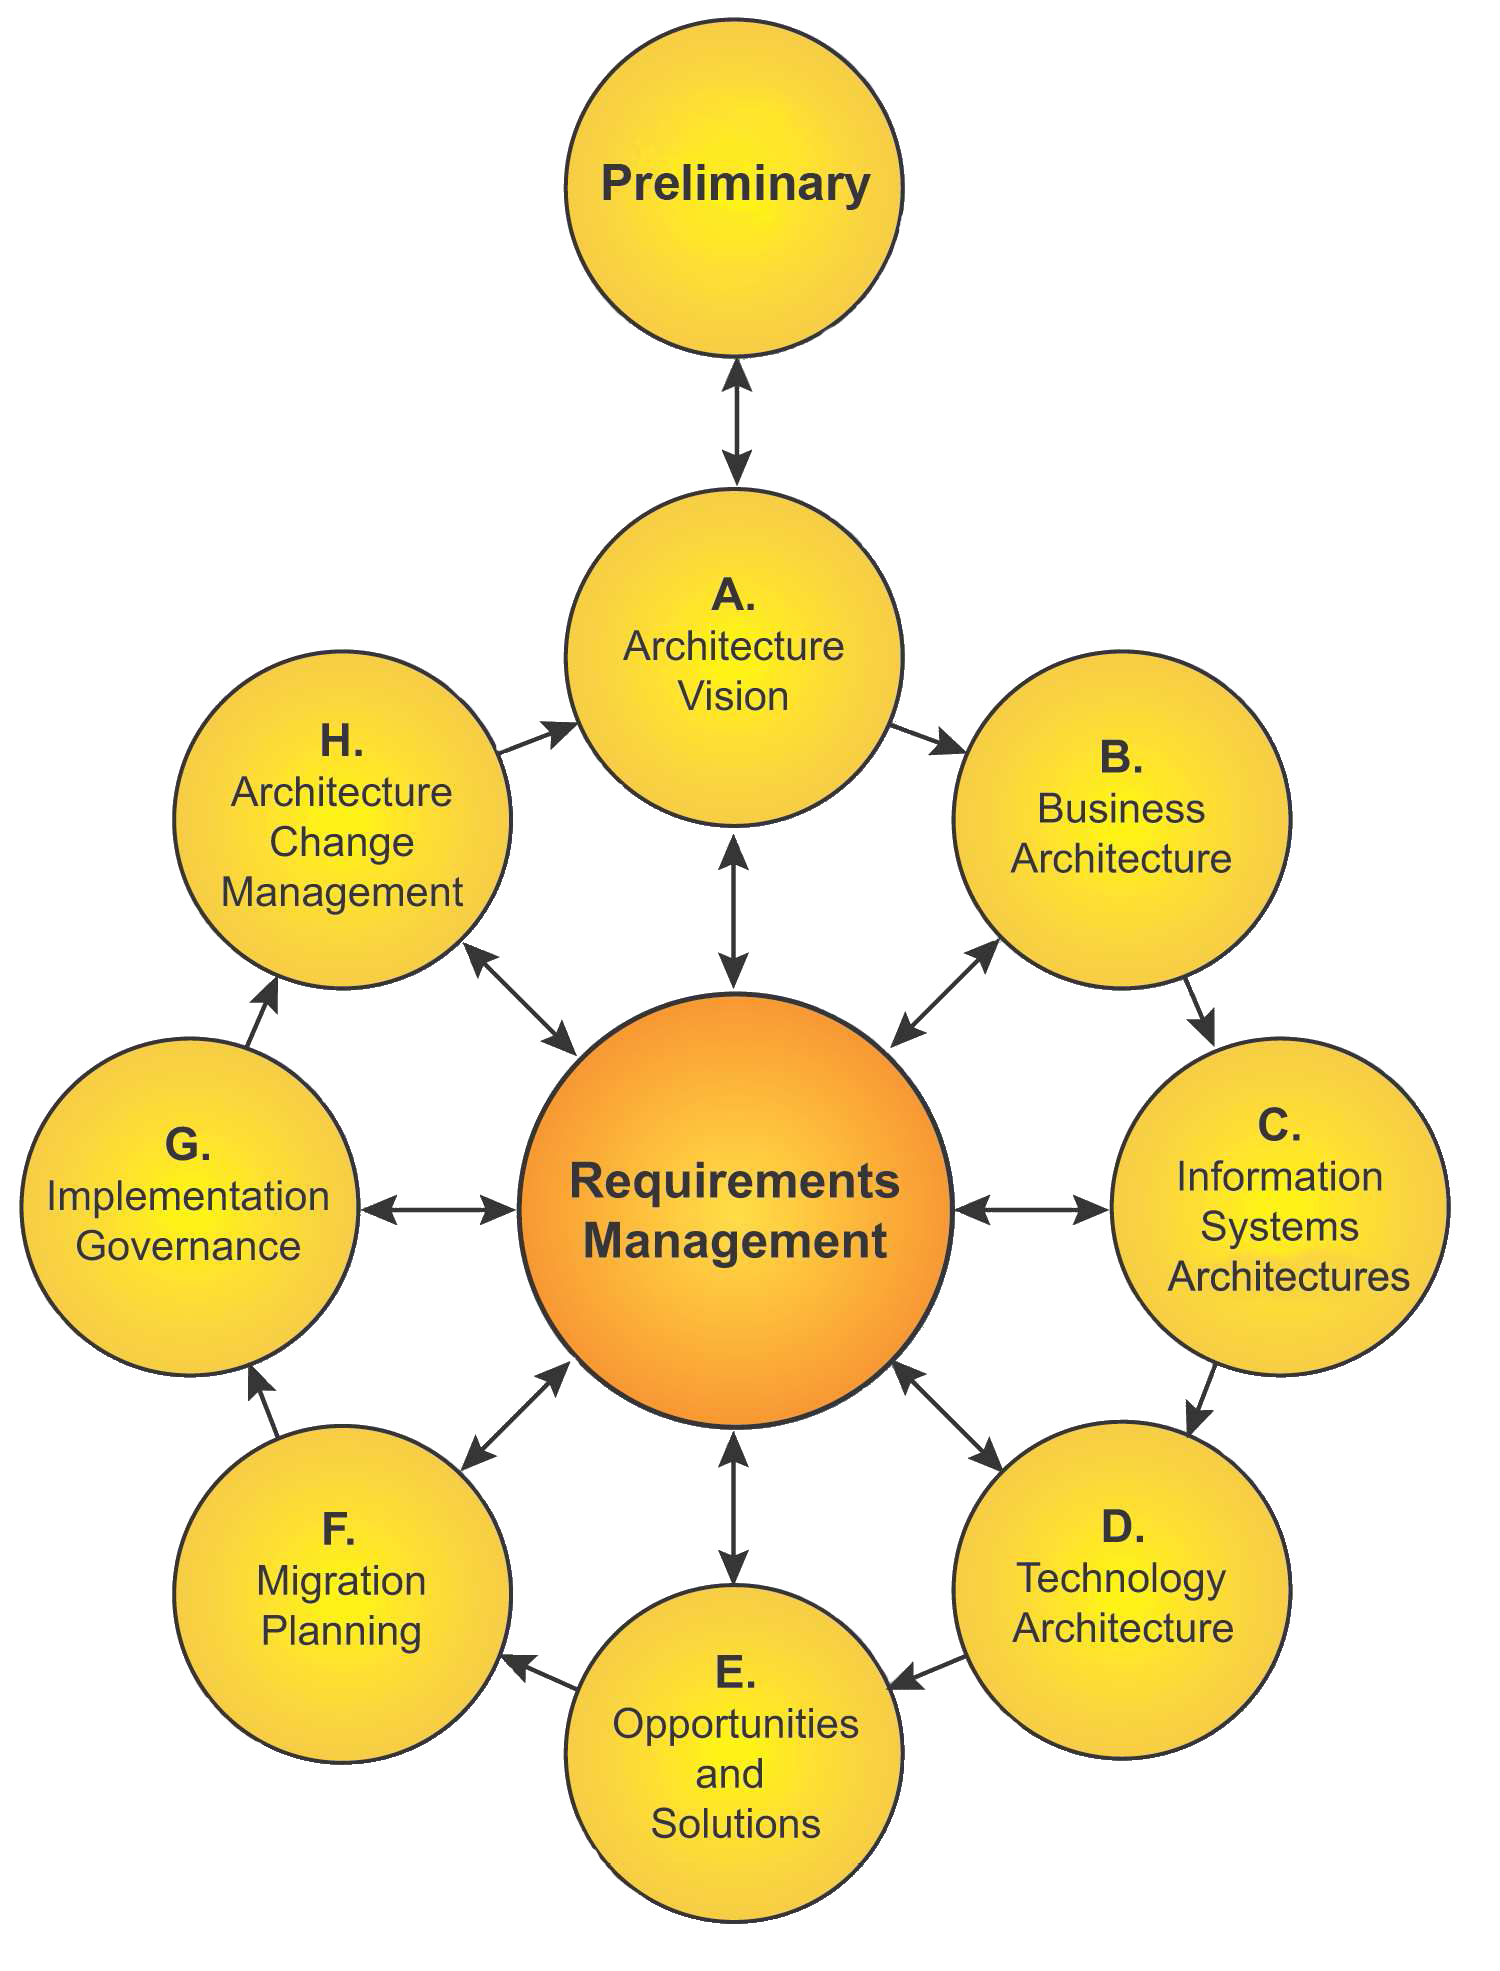
\includegraphics[width=0.8\textwidth]{figures/2_etat_de_l_art_EA/TOGAF9_Wheel.png}
    \end{center}
    \caption{TOGAF Architecture Development Method \protect\cite{togaf2009}}
    \label{fig:TOGAF}
\end{figure}

La méthode \gls{adm} correspond à un processus de conception cyclique. Elle préconise
de piloter l'EA par la gestion des exigences. Les exigences sont dérivées de la
stratégie et des objectifs métier de l'entreprise. Elles sont de ce fait
considérées comme le centre névralgique des activités d'architecture et font le
lien entre les différentes étapes~:de la conception de l'architecture à sa mise
en œuvre comme l'illustre la figure~\ref{fig:TOGAF}. 

La méthode \gls{adm} commence par une phase préliminaire qui consiste à initialiser
ou encore contextualiser l'EA. Pendant cette phase, la disposition de
l'entreprise à engager une démarche d'EA est évaluée et les grands principes
d'EA sont définis en accord avec le métier. Le cycle \gls{adm} se poursuit avec les
huit phases, notées de A à G, relatives à la création des vues métier,
applicative, information et technique. Il s'agit ensuite de planifier le
déploiement de l'architecture avant de l'implémenter. La dernière phase (notée H)
consiste à gérer les changements qui peuvent survenir suite aux évolutions
métier ou technologiques pour assurer une mise à jour continue de
l'architecture. 

Générique, \gls{togaf} peut être appliqué à des entreprises diverses
indifféremment de leurs secteurs d'activité. Flexible et largement paramétrable, ce cadre d'architecturepréconise un ensemble de bonnes pratiques à adapter selon les cas. Il est par exemple possible de recourir au schéma de classification de Zachman dans le
cadre d'une démarche \gls{adm}.

\gls{togaf} comme Zachman laisse aux praticiens la liberté de choisir les langages de
modélisation et le niveau de détail requis pour la conception des vues de
l'architecture. 

\subsubsection{RM-ODP}
\gls{rmodp} est un standard ISO/ITU \footnote{International Organization for Standardization/International Telecommunication Union} qui définit un cadre d'architecture pour la spécification des systèmes distribués ouverts.
Il se réfère au paradigme de l'orienté objet et identifie cinq points de vue~:
\begin{itemize}
\item le point de vue Entreprise, qui décrit les activités métier du système~;
\item le point de vue Information, qui définit l'information traitée par le système et la
façon dont elle est traitée par les différents composants~;
\item le point de vue Traitement, qui spécifie les traitements effectués
par les différents composants en termes de fonctions et en faisant abstraction de toute plate-forme technique~;
\item le point de vue Ingénierie, qui décrit les mécanismes logiciels permettant la
distribution des composants et leur exécution sur les plates-formes d'exécution~;
\item le point de vue Technologie, qui définit les technologies matérielles et logicielles
utilisées pour l’infrastructure d’exécution, leur configuration.
\end{itemize}

\gls{rmodp} préconise de découpler les préoccupations métier des
contraintes liées à une plate-forme technique donnée. En effet, les cinq points de vue sont séparés mais corrélés. Chaque objet d'un point de vue donné correspond à un autre objet dans un autre point de vue.

\gls{rmodp} offre un cadre de référence mais ne préconise pas de méthode d'architecture. Cette correspondance entre les différents points de vue n'est donc pas nécessairement respectée en spécifiant, par exemple, chaque point de vue de façon isolée.
Pour y remédier, EDF R\&D a proposé DASIBAO, une Démarche d’Architecture des
Systèmes d’Information Basée sur RM-ODP. DASIBAO préconise le langage UML dans la
spécification des cinq points de vues qu'il aborde dans l'ordre itératif suivant~:

\begin{center}
Entreprise $\rightarrow$ Information $\rightarrow$ Traitement $\rightarrow$ Ingénierie $\rightarrow$ Technique.
\end{center}

C'est donc par construction que DASIBAO se propose d'assurer la cohérence des
différents points de vue.

\subsubsection{SGAM}

Le \gls{sgam} \cite{uslar2012standardization} adresse l'architecture du Smart Grid en englobant les trois domaines : SI, réseau électrique et réseau de télécommunication. (Le reste à récupérer d'une note H rédigée pour EDF.)


\subsection{Points de vue retenus}
Les cadres d'EA n'utilisent pas tous les mêmes points de vue~: leurs nombres,
leurs noms ainsi que les préoccupations qu'ils adressent varient. Néanmoins,
ces cadres recourent souvent, implicitement ou explicitement, aux points de vue
ci-après.

\begin{description}

    \item[Point de vue métier]:~ce point de vue reflète la vision métier de
    l'entreprise. On y retrouve ses objectifs ainsi que ses processus. Ces
    derniers sont représentés selon la structure organisationnelle de
    l'entreprise en termes d'acteurs internes et externes~;

    \item[Point de vue fonctionnel]:~ce point de vue organise l'entreprise en
    blocs fonctionnels implémentant les processus de la vue métier. Cette
    structuration implique souvent une grande cohérence au sein d'un même bloc
    et une forte décorrélation entre blocs dans un souci de modularité et
    d'évolutivité. À l'échelle d'une entreprise, cette structuration devient
    vite complexe à cause du caractère étendu, transverse et interdépendant des
    processus métier impactés~;

    \item[Point de vue applicatif]:~ce point de vue structure l'entreprise en
    blocs applicatifs. Chaque bloc implémente un ou plusieurs blocs
    fonctionnels. Il est aussi important de spécifier les échanges entre blocs
    applicatifs. Comme pour la vue fonctionnelle, la vue applicative des très
    grandes entreprises souffre souvent du syndrome du plat à spaghetti~:~les
    nombreuses applications fortement couplées deviennent difficiles et
    chères à maintenir~;

    \item[Point de vue technique]:~ce point de vue correspond à
    l'infrastructure technique nécessaire à l'exécution des blocs applicatifs.
    Le point de vue technique spécifie ainsi les machines physiques et liens de
    communication utiles au déploiement des applications informatiques. 

\end{description}

En outre, ces cadres d'architecture sont orientés composants car ils utilisent
des concepts tels que les macros processus, les blocs fonctionnels ou encore
les blocs applicatifs. Les informations sont modélisées soit implicitement et
de manière diffuse à l'intérieur des vues (\gls{togaf}), soit séparément dans une vue
dédiée et décorrélée des autres vues (\gls{rmodp}, \gls{sgam}). Une troisième
méthode consiste à les modéliser sous forme d'aspect pour chaque vue (Zachman,
Archimate).

De plus, ces cadres d'architecture organisent hiérarchiquement les différentes vues en
appliquant \emph{« IT follows business »} comme principe : commencer par la
vue métier et la dériver progressivement jusqu'à l'infrastructure
technique en passant par les fonctions et les applications
\cite{winter2006essential}. 

Les cadres d'architecture sont certes indispensables pour aboutir à une représentation pertinente des composants de l'entreprise mais ne suffisent pas à appréhender la complexité du système entreprise. Pour cela, il est primordiale de disposer d'outils et de méthodes appropriés à l'analyse des modèles d'entreprise obtenus. La section suivante offre un tour d'horizon de l'activité d'analyse en EA. 

\section{Analyse en Architecture d'Entreprise}

La valeur ajoutée de l'EA réside dans sa capacité à adresser le changement en
offrant une vue holistique de l'entreprise. En effet, l'efficacité de
l'entreprise dépend de l'orchestration effective de ses différents composants
et entités plutôt que d'optimisations locales et isolées
\cite{nadler1992organizational}. 

La documentation et la description ne suffisent cependant pas à assurer une
architecture à la fois cohérente et pertinente pour le métier. Les techniques
d'analyse de modèles sont indispensables à l'optimisation globale et effective
d'une architecture \cite{lankhorst2013enterprise}. Les techniques d'analyse de
modèles jouent donc un rôle crucial dans tout processus de changement affectant
l'entreprise en éclairant efficacement la prise de décision. En effet,
l'analyse de l'architecture d'entreprise ne doit pas se résumer pas à la revue
mentale ou manuelle d'une vue d'ensemble étant données la taille et la
complexité des architectures impliquées.

\subsection{Au-delà des modèles «~contemplatifs~»}

Les entreprises recourent aux cadres d'EA pour les guider dans la création et
la maintenance de leurs architectures et pour avoir ainsi une vue globale et
cohérente de leurs stratégies, leurs processus métier et leurs IT 

Les artefacts issus d'une démarche d'EA se résument souvent à un ensemble de
documents utilisés comme supports de communication et comme schéma directeur au
sein de l'organisation \cite{kulkarni_modelling_2013}
\cite{clark_towards_2014}.  Ces modèles fournissent certes un vocabulaire
commun aux différentes parties prenantes mais ne sont	 ni manipulables ni
interprétables par une machine. Ce sont des modèles purement «~contemplatifs~».
Cette terminologie est introduite par Bézivin \cite{bezivin_towards_2001} en qualifiant les modèles de spécification utilisés pendant les premières phases de conception en génie
logiciel. 

Aussi, l'EA s'intéresse-elle d'avantage aux aspects structuraux de
l'entreprise. Pour cette raison, les modèles utilisés, bien qu'offrant
l'abstraction nécessaire pour adresser la complexité de l'entreprise, sont le
plus souvent statiques. Ce genre de modèles ne permet pas d'appréhender les
comportements de l'entreprise et sont donc insuffisants pour éclairer
efficacement les prises de décision au niveau stratégique.

L'EA, à travers les différents cadres d'architecture proposés lors de ces trente
dernières années, a certes contribué à traiter de manière intégrée les
différents aspects d'une entreprise tels que les processus, le personnel, les
services et l'IT. Cependant, la gestion des artefacts issus de l'EA reste un
défi malgré l'existence d'outils sur étagère. En effet, les architectes d'entreprise expérimentés ainsi que les autres parties prenantes impliquées dans les activités
d'architecture sont supposés se fier à leur bon jugement pour créer une
architecture adéquate. 

L'architecture créée est donc correcte par définition et dépend essentiellement
des capacités de l'architecte et de son expertise. Certains travaux proposent de
rendre l'EA moins dépendante de l'expertise de la personne en charge en traduisant les représentations d'architecture en ontologies \cite{sunkle_analyzing_2013}. Les ontologies étant exécutables, permettent en effet de bénéficier des capacités d'analyse des raisonneurs disponibles .

Certaines méthodes d'EA sont accompagnées de langages de modélisation comme le langage
Archimate pour TOGAF. Dans leur quête de généricité, ces langages deviennent rapidement
très larges et difficiles à manipuler. Les modèles produits sont d'autant plus
difficiles à gérer qu'ils ne sont pas manipulables par une machine. L'activité
d'analyse en EA, bien que cruciale, est donc compromise par toutes ces
limitations. Et bien que des modèles et des techniques destinés à l'analyse des
architectures d'entreprise existent, le recours aux modèles exécutables
reste encore marginal dans le domaine de l'EA \cite{kulkarni2013modelling}.

Parmi ces travaux nous citons le langage LEAP \cite{clark2011leap}. Léger, 
générique et exécutable, LEAP est destiné à l'analyse des modèles issus de l'EA 
pour valider l'alignement des modèles métier et IT 

Les deux sections suivantes présentent deux schémas de classification des
approches d'analyse en EA. Le premier est proposé par Lankhorst
\cite{lankhorst2013enterprise} et et le deuxième par Buckl et al. \cite{buckl2009classifying}. Ces schémas de classification nous permettent de (1) comparer entre elles les différentes approches d'analyse recensées dans cet état de l'art et (2) positionner nos travaux.


\subsection{Classification des approches d'analyse selon Lankhorst}

Lankhorst \cite{lankhorst2013enterprise} utilise deux dimensions pour classifier les différentes approches d'analyse d'architecture d'entreprise~:~le type d'analyse et la technique employée. Ceci donne lieu à quatre catégories comme l'illustre la
figure \ref{fig:classLankhorst}. La première dimension fait la distinction
entre deux types d'analyse.

\begin{description}
    \item[L'analyse fonctionnelle] concerne les aspects fonctionnels de
    l'architecture. Elle permet par exemple de valider la structure ou de
    comprendre le comportement d'une architecture.

    \item[L'analyse quantitative] concerne les aspects non fonctionnels de
    l'architecture comme la performance ou le coût.
\end{description}

\begin{figure}[!ht]
    \begin{center}
        \begin{tikzpicture}
    \draw[<->] (-1.5,0) node[anchor=east] {Analytique} -- (1.5,0) node[anchor=west] {Simulation};
    \draw[<->] (0,-1.5) node[anchor=north] {Fonctionnelle} -- (0,1.5) node[anchor=south] {Quantitative};
\end{tikzpicture}

    \end{center}
    \caption{Classification des approches d'analyse selon Lankhorst 
    \protect\cite{lankhorst2013enterprise}}
    \label{fig:classLankhorst}
\end{figure}

La deuxième dimension identifie deux techniques pouvant être employées pour 
l'analyse fonctionnelle ou quantitative~:

\begin{description}

    \item[La technique de simulation] des modèles revient à les exécuter. La simulation 	dans le cas de l'analyse fonctionnelle est utilisée
    pour mieux appréhender les aspects dynamiques d'une architecture. La
    simulation quantitative permet de mesurer des paramètres quantitatifs tel
    que le temps d'exécution d'un processus métier par exemple à travers
    plusieurs itérations de la simulation. 

    \item[La technique analytique] est plus formelle que la simulation.  Ici le
    terme analytique signifie plutôt «~mathématique~». Cette technique est plus
    efficace que la simulation quantitative pour fournir des indicateurs de
    performance. 

\end{description}

\subsection{Classification des approches d'analyse selon Buckl}
	
Le schéma de classification de Lankhorst \cite{lankhorst2013enterprise} offre un premier aperçu des différentes approches d'analyse d'architecture cependant il ne révèle pas toutes les variantes et les subtilités d'une démarche d'analyse en EA. Nous considérons donc les travaux de Buckl et al. \cite{buckl2009classifying} qui définissent un système de classification plus détaillé. Ce système classification peut même être considéré comme un cadre d'analyse d'architectures.

Buckl et al. \cite{buckl2009classifying} font intervenir cinq dimensions pour catégoriser
les approches d'analyse d'architecture d'entreprise. Ces dimensions sont illustrées par la figure~\ref{fig:classBuckl}.

\begin{figure}[!ht]
	\begin{tikzpicture}[scale=0.9]
    \path[
        mindmap,
        every node/.style={concept, color=black},
        level 1/.append style={sibling angle=360/5, distance=1cm},
        grow cyclic]
    node {L'analyse en Architecture d'Entreprise}
    child {
        node {Sujet de l'analyse}
        child {
            node {Structure}
        }
        child {
            node {Dynamique}
        }
        child {
            node {Statistiques}
        }
    }
    child {
        node {Référence temporelle}
        child {
            node {Ex post}
        }
        child {
            node {Ex ante}
        }
    }
    child {
        node {Techniques}
        child {
            node {Basée sur les experts}
        }
        child {
            node {À base de règles}
        }
        child {
            node {À base d'indicateurs}
        }
    }
    child {
        node {Préoc\-cupations}
        child {
            node {Fonction\-nelles}
        }
        child {
            node {Non Fonctionnelles}
        }
    }
    child {
        node {Auto\-référentialité}
        child {
            node {Aucune}
        }
        child {
            node {un niveau}
        }
        child {
            node {plusieurs niveaux}
        }
    };
\end{tikzpicture}

	\caption{Schéma de classification des approches d'analyse selon Buckl et al. \protect\cite{buckl2009classifying}}
	\label{fig:classBuckl}
\end{figure}


\subsubsection{Sujet de l'analyse}

L'analyse peut concerner trois aspects différents de l'architecture~:~sa
structure, son comportement dynamique ou son comportement statistique. D'abord,
l'analyse de la structure est nécessaire pour appréhender la complexité
structurelle des entreprises. Celle-ci est due à la densité des interconnexions
entres ses composants. Ensuite, la complexité de la structure de l'entreprise
induit une complexité au niveau de son comportement d'où la nécessité
d'analyser l'aspect comportemental de l'architecture pour évaluer l'impact
d'une anomalie sur le déroulement d'un processus par exemple. Enfin, l'analyse et
l'agrégation des mesures statistiques provenant du comportement offrent une
meilleure compréhension de l'architecture.

\subsubsection{Référence temporelle}

L'analyse peut se porter sur l'architecture d'une entreprise dans son état
courant ou telle qu'elle est planifiée. Une analyse \textit{ex post} concerne
les modèles d'une architecture déjà mise en place alors qu'une analyse
\textit{ex ante} se réfère à différents scénarios élaborés pour une future
implémentation.

\subsubsection{Technique d'analyse}

Les techniques d'analyse employées peuvent s'appuyer sur des experts, sur des
règles ou sur des indicateurs. Les analyses orientées experts sont les moins
formelles et dépendent du niveau d'expertise de l'expert impliqué. Cette technique d'analyse est certes chronophage mais c'est celle qui offre le plus de flexibilité. Les résultats d'une telle analyse prennent la forme de conseils
concrets ou d'idées et de directives générales concernant l'architecture en
question.

Les techniques d'analyse s'appuyant sur des règles sont plus formelles que
celles s'appuyant sur des experts et peuvent être plus facilement automatisées.
Ces règles décrivent les modèles de conception que l'architecture doit
respecter ou éviter. 

Les techniques d'analyse s'appuyant sur des indicateurs sont encore plus
formelles que les deux précédentes et servent à évaluer en les quantifiant
certaines propriétés de l'architecture. Les résultats d'une telle analyse
doivent cependant être interprétés avec prudence car ils dépendent d'hypothèses
souvent amenées à évoluer.

\subsubsection{Préoccupations de l'analyse}

Buckl et al. \cite{buckl2009classifying} font la différence entre les analyses fonctionnelles et les analyses non
fonctionnelles à la manière de Lankhorst \cite{lankhorst2013enterprise}. L'analyse fonctionnelle évalue si l'architecture remplie les fonctions métier de l'entreprise telles que la production ou la vente. L'analyse non fonctionnelle évalue des aspects comme le
temps d'exécution d'un processus ou le coût de l'implémentation et de
maintenance d'une architecture. Contrairement à Lankhorst \cite{lankhorst2013enterprise}, Buckl et al. \cite{buckl2009classifying}
emploient le terme \textit{non fonctionnelle} plutôt que \textit{quantitative}
en arguant que certains aspects non fonctionnels telle que la sécurité peuvent être analysés de manière non quantitative. 

\subsubsection{Autoréférentialité}

Les personnes en charge de l'EA peuvent faire partie
l'architecture créée car appartiennent aussi à l'entreprise. Qui plus est,
l'activité de décrire et de planifier l'architecture de l'entreprise peut
elle-même être décrite et planifiée et fait par conséquent partie de l'activité
d'EA. Selon Buckl et al.  \cite{varela1974autopoiesis}
l'entreprise est en effet un système vivant capable de faire sa propre autopsie
\cite{varela1974autopoiesis}.

L'analyse peut considérer un seul niveau d'autoréférentialité en intégrant les
activités de management d'architecture. Une analyse à plusieurs niveaux
d'autoréférentialité incorporent des activités de meta-management
d'architecture comme par exemple la gouvernance des activités de management
d'architecture.  L'autoréférentialité augmente la complexité de l'analyse. Peu de
travaux considèrent des niveaux d'autoréférentialité multiples
\cite{smook2014executable}. Nous citons parmi celles-ci les travaux de
\cite{metrailler_evolis_2014} qui traitent la gestion et la gouvernance
d'architecture en définissant des stratégies d'évolution pour les architectures
actuelles vers les architectures cible dans un framework dédié. 


\subsection{Analyse de la structure}

\subsubsection{Finalités}

Maintenir une cohérence entre l'infrastructure informatique de l'entreprise
avec ses processus métier est au cœur des activités
d'EA\cite{lankhorst2013enterprise}. L'objectif de cet alignement est
d'améliorer l'efficacité de l'entreprise et de maximiser ses bénéfices.
L'alignement métier/IT reste une problématique cruciale pour les entreprises
qui s'appuient sur les technologies de l'information dans la réalisation de leurs
objectifs métier \cite{kaisler_enterprise_2005}. Zachman affirme même que
seules les entreprises capables d'aligner rapidement leurs SI à leurs
stratégies métier sont en mesure de survivre dans un environnement hautement
concurrentiel \cite{zachman1997enterprise}.
	
Pour Lankhorst \cite{lankhorst2013enterprise}, l'EA a pour vocation d'offrir une vue
générale et homogène du métier de l'entreprise, de son patrimoine applicatif,
de son infrastructure technique et de son évolution pour en faciliter
l'analyse via un ensemble cohérents de principes, méthodes et modèles. De plus, l'EA explicite et documente les relations entre les processus métier et
l'IT de l'entreprise \cite{kaisler_enterprise_2005}. 
	
En offrant une vision globale de l'entreprise et en documentant les
relations entre ses différents composants, l'EA est un outil incontournable
pour les architectes dans leur quête d'alignement métier/IT. Cependant, les
méthodes et techniques actuelles offerts par l'EA ne suffisent pas à atteindre
cet objectif \cite{barn2013enterprise} car :
\begin{itemize}
\item les processus métier, les technologiques, les structures organisationnelles
ainsi que l'environnement sont en constante évolution. Les changements sont si
rapides et nombreux qu'un réel alignement relève du vœux pieux
\cite{lankhorst2013enterprise}. L'alignement métier/IT correspond plutôt un
idéal kantien vers lequel l'entreprise doit tendre à défaut de le réaliser
complètement~;

\item l'architecture en tant que discipline tient d'avantage de l'art que de la science. En effet, l'architecte d'entreprise analyse souvent de la documentation (tels que des tableurs Excel ou des
illustrations Power Point) même si quelques logiciels permettent désormais de
visualiser ces modèles. Cette tâche devient rapidement ardue dès qu'il s'agit
de grandes entreprises dont l'important patrimoine applicatif s'apparente à un
plat de spaghetti.
\end{itemize}

\subsubsection{Approches d'analyse de la structures existantes et leurs limites}
	
Les modèles exécutables peuvent assister les architectes d'entreprise à
surmonter les obstacles cités ci-dessus. Les modèles exécutables augmentent
l'agilité de l'architecture en détectant automatiquement les incohérences dès
les premières phases de conception. 
	
Les approches de modélisation en EA recourent souvent à des langages
semi-formels qui ne permettent pas de vérifier dynamiquement et automatiquement
certaines propriétés requises pour l'architecture comme la cohérence entres
vues. Partant de ce constat, \cite{sunkle_analyzing_2013} proposent de recourir
aux ontologies tirant ainsi profit des raisonneurs disponibles pour analyser la
structure des architecture d'entreprise. Ils arrivent à analyser l'impact du
changement ou encore les relations et dépendances entre les opérations métier
et les applications informatiques de l'entreprise. Cependant, les architectes
d'entreprise sont peu familiarisés avec les ontologies. Les modèles
d'architecture sont donc traduits en ontologies, risquant de faire
apparaître un gap sémantique entre les modèles utilisés pour la représentation
de l'architecture et les ontologies utilisées pour mener l'analyse.
	
La diversité des acteurs impliqués dans l'EA comme l'architecte d'entreprise,
le manager ou encore l'ingénieur IT engendre une hétérogénéité au niveau des
modèles utilisés. \cite{bruneliere2013support} proposent de créer un mapping
entre des modèles hétérogènes (tels que des tableurs Excel, de la documentation
ou des bases de données). Pour cde faire, ils recourent à des modèles manipulables par machine et mettent à profit les techniques de tissages de modèles issus de l'IDM. Ces
travaux adressent l'hétérogénéité des modèles et offrent une vue intégrée
de l'architecture de l'entreprise en l'adaptant aux acteurs concernés. Mais elle ne permet pas de mener des analyses concernant l'impact du changement par exemple. 

	
\subsection{Analyse du comportement}

\subsubsection{Finalités}

Pour Shannon \cite{shannon1975systems}, la simulation est «~un processus
consistant à modéliser un système réel et à mener des expérimentations sur le
modèle obtenu dans le but de comprendre le comportement du système et/ou
d'évaluer différentes stratégies concernant son fonctionnement~».  Quel qu'en
soit le domaine d'application, la simulation est un moyen d'apprécier les choix
des concepteurs sur le comportement du système modélisé. Elle peut se traduire par
par l'animation d'un modèle (représentant notre perception du système,
qu'il soit existant ou à construire) et l'étude du comportement de ce modèle en
fonction des variables en entrée. 

La simulation des architectures d'entreprise permet de modifier localement des stratégies
et d'observer l'impact de ces modification sur le comportement globale du système \cite{buckl2008towards}. La simulation des architectures d'entreprise est d'autant plus cruciale dans le contexte des Smart Grids. Ces derniers sont en constante et rapide transformation~:~évolution des cadres législatifs, apparition de nouveaux partenaires, hétérogénéité des interactions avec les clients finaux (les compteurs intelligents, Internet, les téléphones ou encore les tablettes). 

Ainsi, le recours à la simulation dès les premières phases du cycle de vie des
architectures d'entreprise dans le contexte des Smart Grids augmente leur évolutivité en apportant une aide supplémentaire à leur validation. La simulation des modèles facilite leurexploration par les experts métier et lève les ambiguïtés engendrées par les
modèles purement contemplatifs. Elle permet en outre un prototypage rapide et
une analyse itérative des modèles par les parties prenantes tels que les
architectes d'entreprise, les expert métier, les analystes ou les architectes
IT. 

\subsubsection{Approches de simulation existantes et leurs limites}

\cite{manzur2015xarchimate} recensent quatorze approches d'analyse
d'architectures d'entreprise et les classent selon les quatre dimension du
schéma de classification de Lankhorst \cite{lankhorst2013enterprise} (précédemment illustré par la figure
\ref{fig:classLankhorst}). Seulement quatre approches parmi les quatorze
recourent à la simulation comme outil d'analyse d'une architecture
d'entreprise.

Le nombre limité d'approches utilisant la simulation pour l'analyse
d'architecture d'entreprise est du au fait que l'EA est initialement conçue
comme une description statique des composants essentiels de l'entreprise et de
leurs interconnexions \cite{hoffman2013enterprise}. Les cadres d'EA standards
ne prennent pas en compte les informations nécessaires pour analyser les
aspects comportementaux d'une entreprise et mettent d'abord l'accent sur ses
aspects structuraux tels que les liens entre les processus et les applications
métier. Il en résulte que les outils d'EA n'adressent souvent que les aspects
statiques de l'entreprise car ils se basent sur les mêmes cadres d'architecture.

Buckle et al. \cite{buckl2009classifying} classifient les approches d'analyse d'architecture existantes selon leur propre système de classification illustré par la figure \ref{fig:classBuckl}. Nous tirons le même constat que pointe l'état de l'art de l'analyse en EA de \cite{manzur2015xarchimate}. 

Dans le présent état de l'art, nous nous intéressons donc aux travaux qui analysent la
dimension dynamique d'une architecture d'entreprise. Parmi ces approches,
celles développées par \cite{glazner2011enterprise},
\cite{ludwig2011organizational} et \cite{manzur2015xarchimate} soulignent
l'importance de simuler le comportement d'une architecture d'entreprise. 

Glazner \cite{glazner2011enterprise} propose une approche de simulation hybride pour
évaluer le comportement d'une entrepris en combinant une simulation à
événements discrets et une simulation multi-agents.
Il met à profit les capacité d'abstraction de l'EA pour adresser la complexité d'un système telle que l'entreprise et s'en sert
comme socle pour structurer les modèles de simulation. Les
techniques et les langages utilisés pour la simulation sont décorrélés des
langages de représentation utilisés par les architectes d'entreprise entrainant
ainsi un gap sémantique entre l'aspect statique de l'entreprise (les composants
de l'entreprise et leurs relations) et son aspect dynamique (le comportement
des composants). 

Ludwig et al. \cite{ludwig2011organizational} simulent une architecture d'entreprise en
fonction de la configuration organisationnelle d'une entreprise. Ils
développent ainsi un langage exécutable pour décrire les relations entre des
concepts de l'ordre organisationnels comme l'entité, le rôle
qu'elle joue, les services qu'elle procure et les processus dans lesquels elle
intervient. La méthode et l'outil développés permettent de reconfigurer les
modèles organisationnels lors de l'exécution. Ces travaux n'adressent cependant
que la vue métier et une partie de la vue fonctionnelle d'une architecture
d'entreprise.

Manzur et al. \cite{manzur2015xarchimate} proposent une plateforme de simulation qui s'appuie sur deux métamodèles différents~:~un premier métamodèle, correspondant au
langage Archimate, pour spécifier les composants structurels de l'architecture
et un deuxième métamodèle complémentaire pour spécifier les comportements des
composants structurels. Les modèles sont ensuite simulés afin d'observer le
comportement de l'architecture et de l'évaluer selon les indicateurs établis.
Cependant cette approche évalue uniquement les aspects non fonctionnels d'une
architecture d'entreprise.

%La modélisation c'est pour abstraire
%Pour simuler on a besoin de détails 
%\cite{de2005enterprise} : dynamique par xlm 
